\chapter{Detail Experiments on \ac{DPRST}}

The main steps of our approach are illustrated in \figref{fig:Apparatus}; a \ac{VHR} orthorectified image is provided by our sponsor and the approximate trajectory of a sidewalk is acquired from a \ac{GIS} such as \ac{OSM}.
Alternately, an approximate trajectory could be marked by a person to digitize the sidewalk quickly. 
The initial trajectory is re-sampled and used to warp a portion of aerial image so that the trajectory is mapped to a straight, horizontal line which we call a \textit{ribbon image}. 
We use a modest assumption that colors near the center of the ribbon image are more likely to be on a walking path in order to build a probability-density estimate for walking path materials. 
Based on the probability estimate at each pixel, we construct a single ribbon with priors that control the rate of change of thickness and direction of the ribbon. 
Finally, the boundaries are warped back onto the original reference frame. 
In this section we elaborate the process of generating a ribbon image, estimating the probability that a color belongs to the same material as a walking path, and the construction of a smooth ribbon image based on the resulting probabilities. 

\begin{figure}[H]
\begin{center}
\includegraphics[width=0.8\textwidth]{Figures/diagram6.png}
\caption[Framework Overview]{Our approach adopted to predict precise boundaries for ribbon-like features. Where black line indicated a sidewalk's geometric information, and red lines shown our result for the sidewalk boundaries.
 From (a) to (f), the 6 step approach introduce 
(a) input map, 
(b)~initial trajectory, 
(c)~ribbon image generation, 
(d)~density Estimation for pixels, 
(e)~the result from our \ac{DP} solution, 
(f)~the output result.}
\label{fig:Apparatus}
\end{center}
\end{figure}

\section{Validate Initial Trajectory}

\begin{figure}[H]
\centering 
\includegraphics[width=\textwidth]{Figures/arizon_center.png}
 \caption[Demonstration on Arizona Center]{
Ground-truth data for a part of Pheonix, Arizona. All sidewalk \ac{GIS}
information is shown in Orange.}
\label{fig:arizon_center}
\end{figure}


It's challenging since the geometric accuracy was not precise,
 which could cause performance issue since we rely on this 
 information to segment the sidewalk part from maps for the next step. 
To ensure data accuracy, as shown in figure \ref{fig:arizon_center},
 we spent days marking all sidewalks and their precise boundaries 
 in Arizona Central for initial experiments. 
We can locate each sidewalk by using the geometric information 
and saved them into separate files. 

\section{Warping an Input Image}

We take as input an image $\InputImage{}$ and a trajectory $\InputTrajectory{}=\langle \vec{p}_0,
\vec{p}_1,\dots,\vec{p}_m\rangle$ where each $\vec{p}_i=(x_i, y_i)^T$ is a point on the initial
estimate of a ribbons trajectory (re-sampled and smoothed). Further, we are able to estimate
unit-length tangent vectors $\vec{u}_i$ and their perpendiculars $\vec{v}_i$; for example by using
the secant method
\begin{align}
  \vec{u}_i &= \frac{\vec{p}_{i+1}-\vec{p}_{i-1}}{\|\vec{p}_{i+1}-\vec{p}_{i-1}\|} \\
  \vec{v}_i &= \left(\begin{array}{cc}
       0  & 1 \\
       -1 & 0
  \end{array} \right) \vec{u}_i
\end{align}
where the endpoints are repeated. 
We define the warped ribbon-image $\RibbonImage{}$ so that $\RibbonImage{[i,j]}=\InputImage{}(\vec{p}_i+ j \vec{v}_i)$. 
We use the convention that square-brackets to indicate discrete indices and rounded parenthesis indicate interpolated samples. 
An example of the process is shown in \figref{fig:Sample_Sidewalk_4} and \figref{fig:Apparatus}(c). 

\begin{figure}[H]
    \centering
    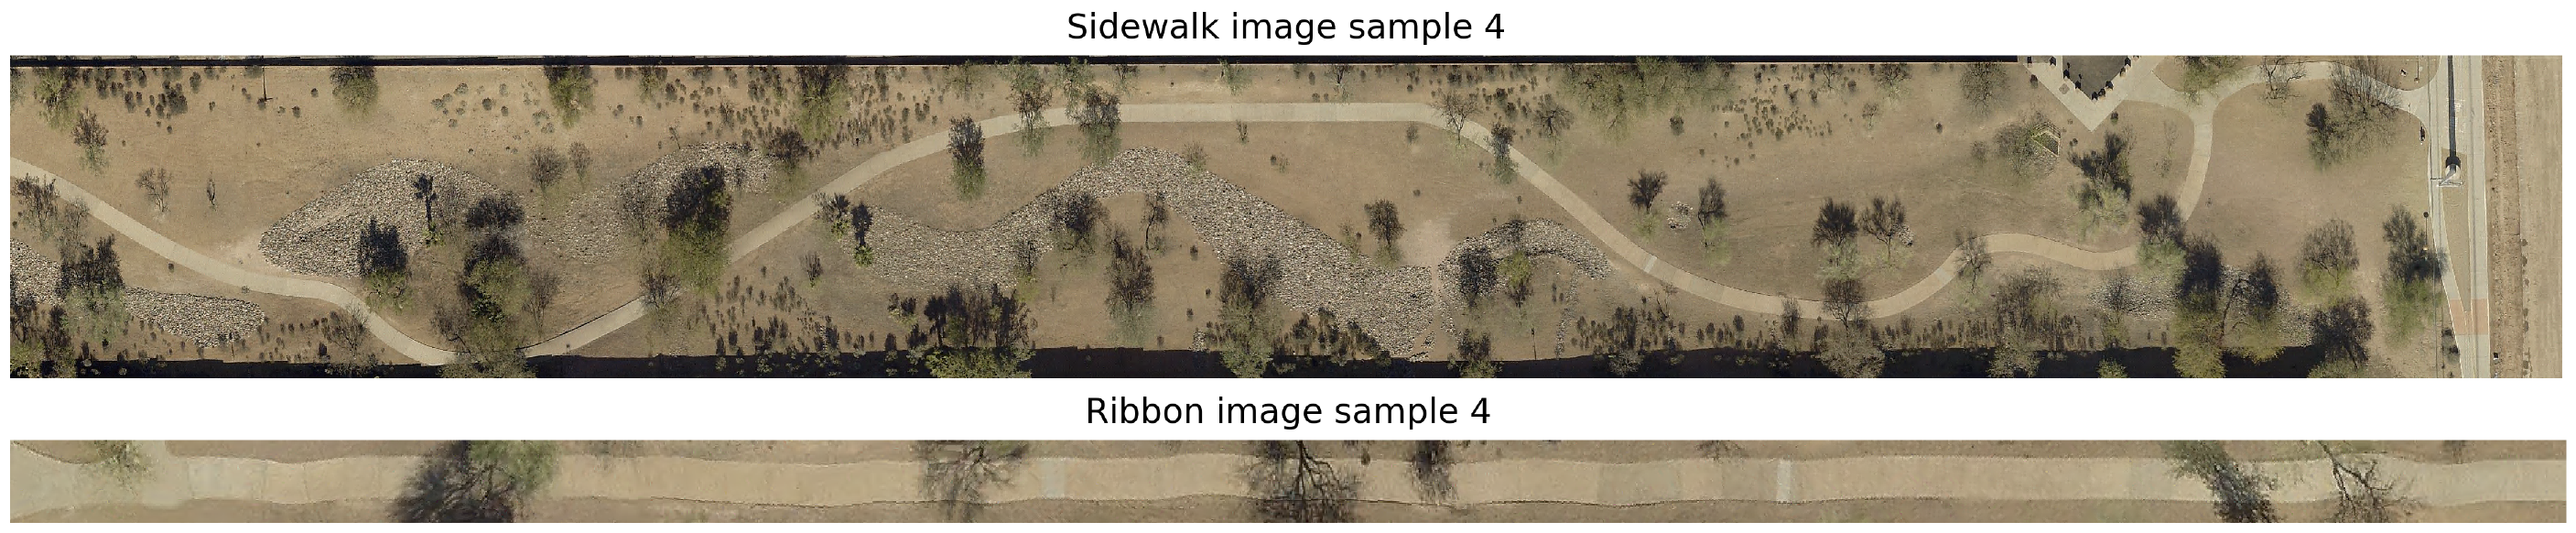
\includegraphics[width=\textwidth]{Figures/Sample4_needed.png}
    \caption[Sample Sidewalk 1]{A ribbon image straighten output which used the previous process from figure \ref{fig:StraightenProcess} to convert an original image into ribbon image .}
    \label{fig:Sample_Sidewalk_4}
\end{figure}

% \begin{figure}[ht]
%     \centering
%     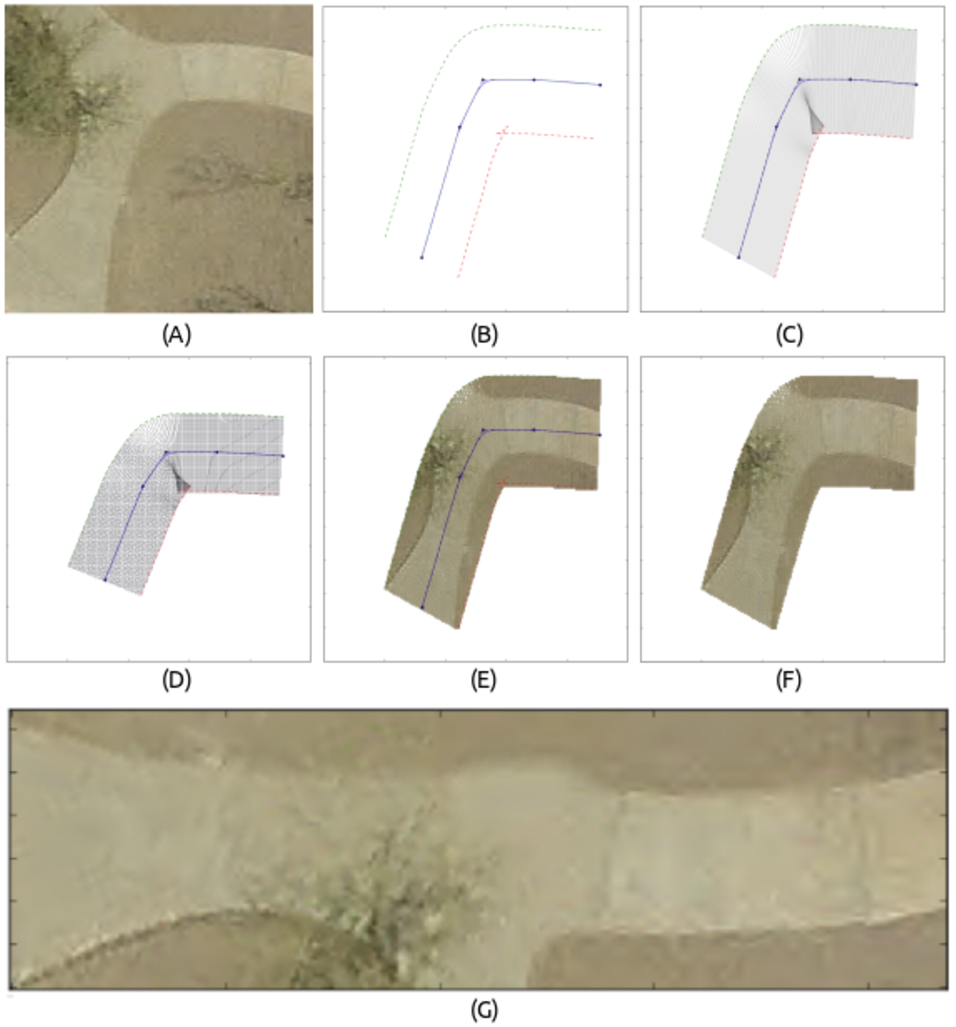
\includegraphics[width=0.95\columnwidth]{Figures/straghten.pdf}
%     \caption[Ribbon Image Generation]{Ribbon image generating process: (a) raw input $\InputImage{}$, (b) we densely resample and smooth the trajectory using $\MaxRadius{}$ iterations of Laplacian smoothing and show the locations of warped pixels of $\RibbonImage{}$ within $\pm \MaxDistance{}$;  (c) the warped ribbon image $\RibbonImage{}$ shown in the original reference frame and  (d) the generated the ribbon image (shown transposed to fit in the figure).}
%     \label{fig:StraightenProcess}
% \end{figure}

% \begin{figure}[ht]
%     \centering
%     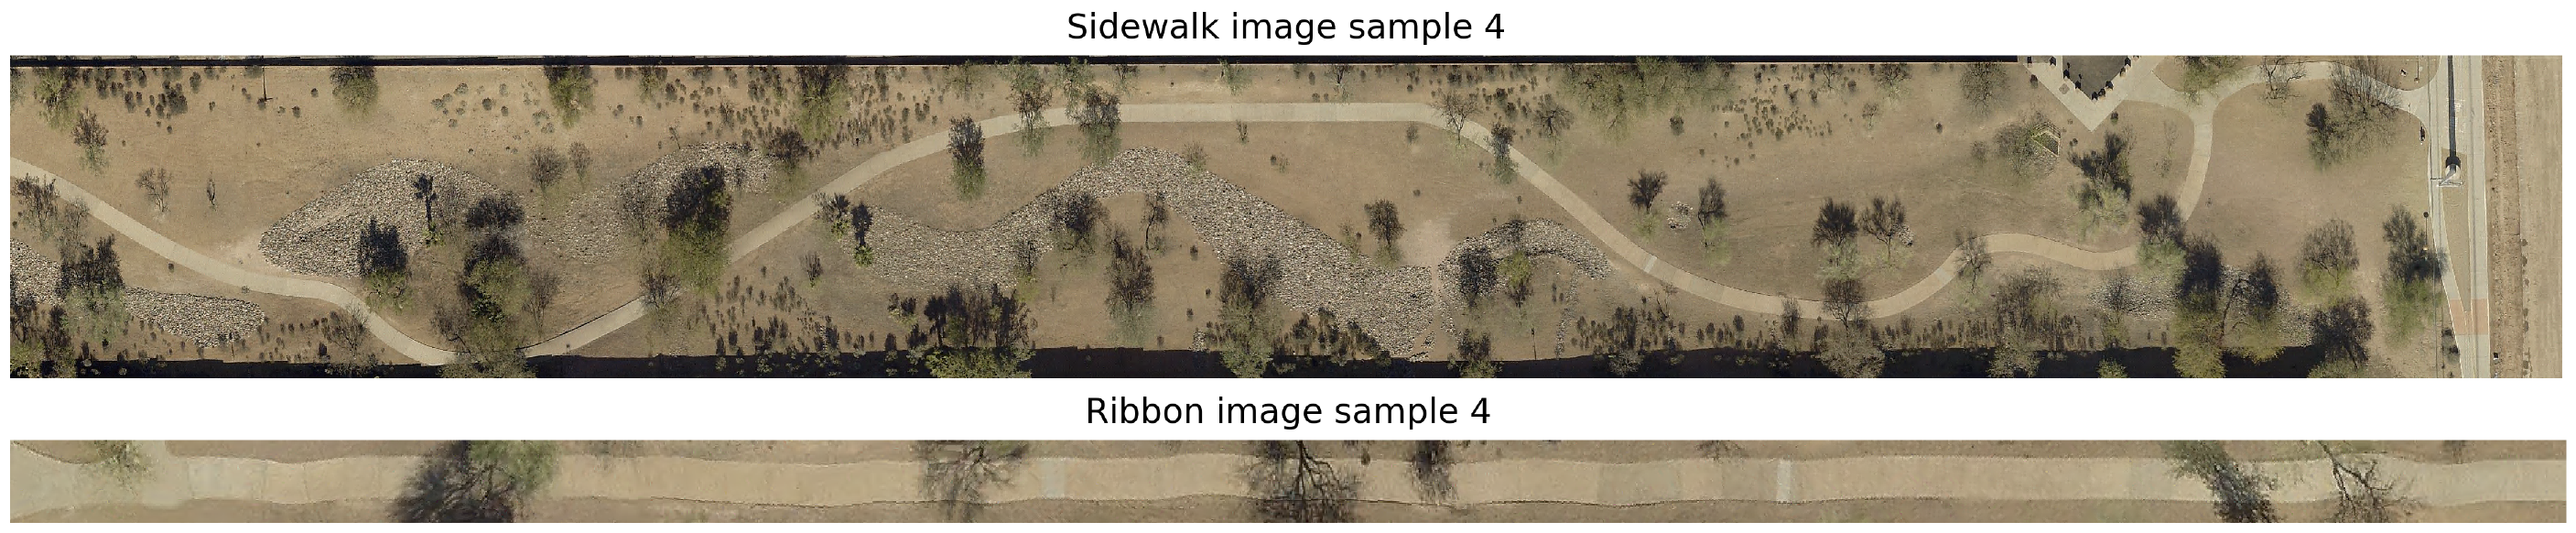
\includegraphics[width=0.95\columnwidth]{Figures/Sample4_needed.png}
%     \caption[Sample Sidewalk]{A ribbon image; the original image $\InputImage{}$ (top) was warped so that the trajectory is a straight line to create a ribbon image $\RibbonImage{}$ (bottom), shown transposed.}
%     \label{fig:Sample_Sidewalk_4}
% \end{figure}

We develop a way to convert the given sidewalk into a ribbon image. 
As shown in figure \ref{fig:StraightenProcess}, we use the previous outcome (A) from the last step as input and connected all coordinate points data as the mid-line for the sample sidewalk. 
Then we apply a smooth function that we created to smooth the mid-line, so the shape of mid-line fits better to the actual sidewalk shape(B). 
We generate two parallel line as offsets on each side of the mid-line with a distance of twice the average width in between. 
Ideally even the mid-line is not perfectly laying on the middle, we would still fit the whole sidewalk into the ribbon image. 
For each point on the mid-line, we connect the corresponding points on both offsets to get the movement of the sidewalk and recorded them(C, D), we generate the straightened ribbon image by using the color data from each pixel in the points set that we record earlier(E). 
The image data in between each offset, with constant image width could be retrieved after that (F).
Then we reshape the image data to generate the ribbon image(G). 
Figure \ref{fig:Sample_Sidewalk_2} shows the complete ribbon-image output result on sample sidewalk. We separate it into parts to show better detail. 

\begin{figure}[H]
    \centering
    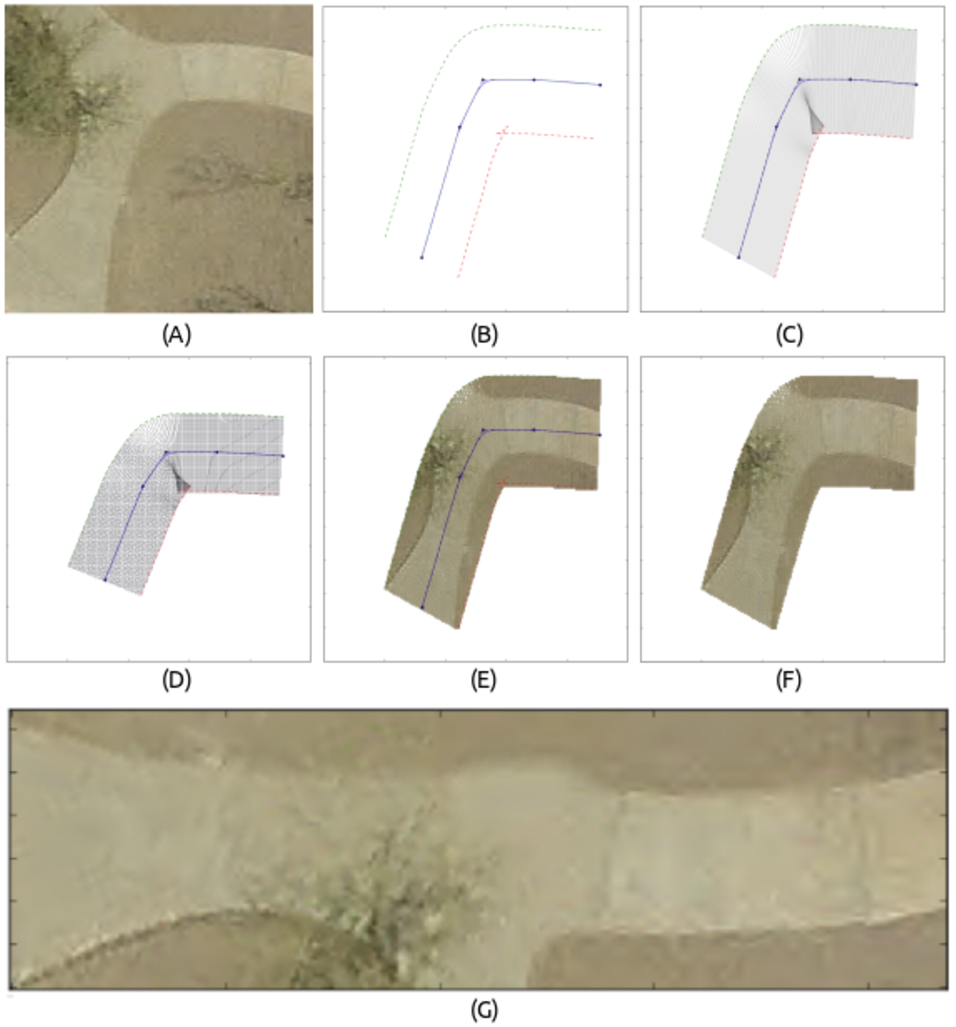
\includegraphics[width=\textwidth]{Figures/straghten.pdf}
    \caption[Ribbon Image Generation]{Ribbon image generating process: from sub-figures A to G, we showed the step by step process to generate ribbon-image from a partial sidewalk. From raw input (A), we smoothed mid line and generated parallel off-site (B). Generated pixels (C) and connected each pixel to its correspond color data from the raw input (D). After gathered pixel data (E), we removed mid-line (F) and generated the ribbon image(G).}
    \label{fig:StraightenProcess}
\end{figure}

\begin{figure}
    \centering
    \includegraphics[width=0.95\textwidth]{Figures/sample2_demo.png}
    \caption[Sample Sidewalk 2]{A ribbon image straighten output on sample sidewalk, row 1 shows the original input, row 2 to 5 show the ribbon image output separate into parts.}
    \label{fig:Sample_Sidewalk_2}
\end{figure}

\section{Density Estimation}\label{sec:density-estimation}
We aim to find a new trajectory $\OutputTrajectory{}[0\dots m]$ and radius $\OutputRadius{}[0\dots m]$ that are most likely given an input image. We first must estimate the probability of observing a color within the ribbon.  
Given an input image $\RibbonImage{}$, let $\Pr(R|\Color{},\theta)$ denote the probability that a pixel is a part of a ribbon given an observed color $\Color{}$ and set of learnable parameters $\theta$. 
We aim to estimate parameters $\theta$ that maximize the likelihood of our \textit{initial} path. 

\begin{figure}[H]
    \centering
    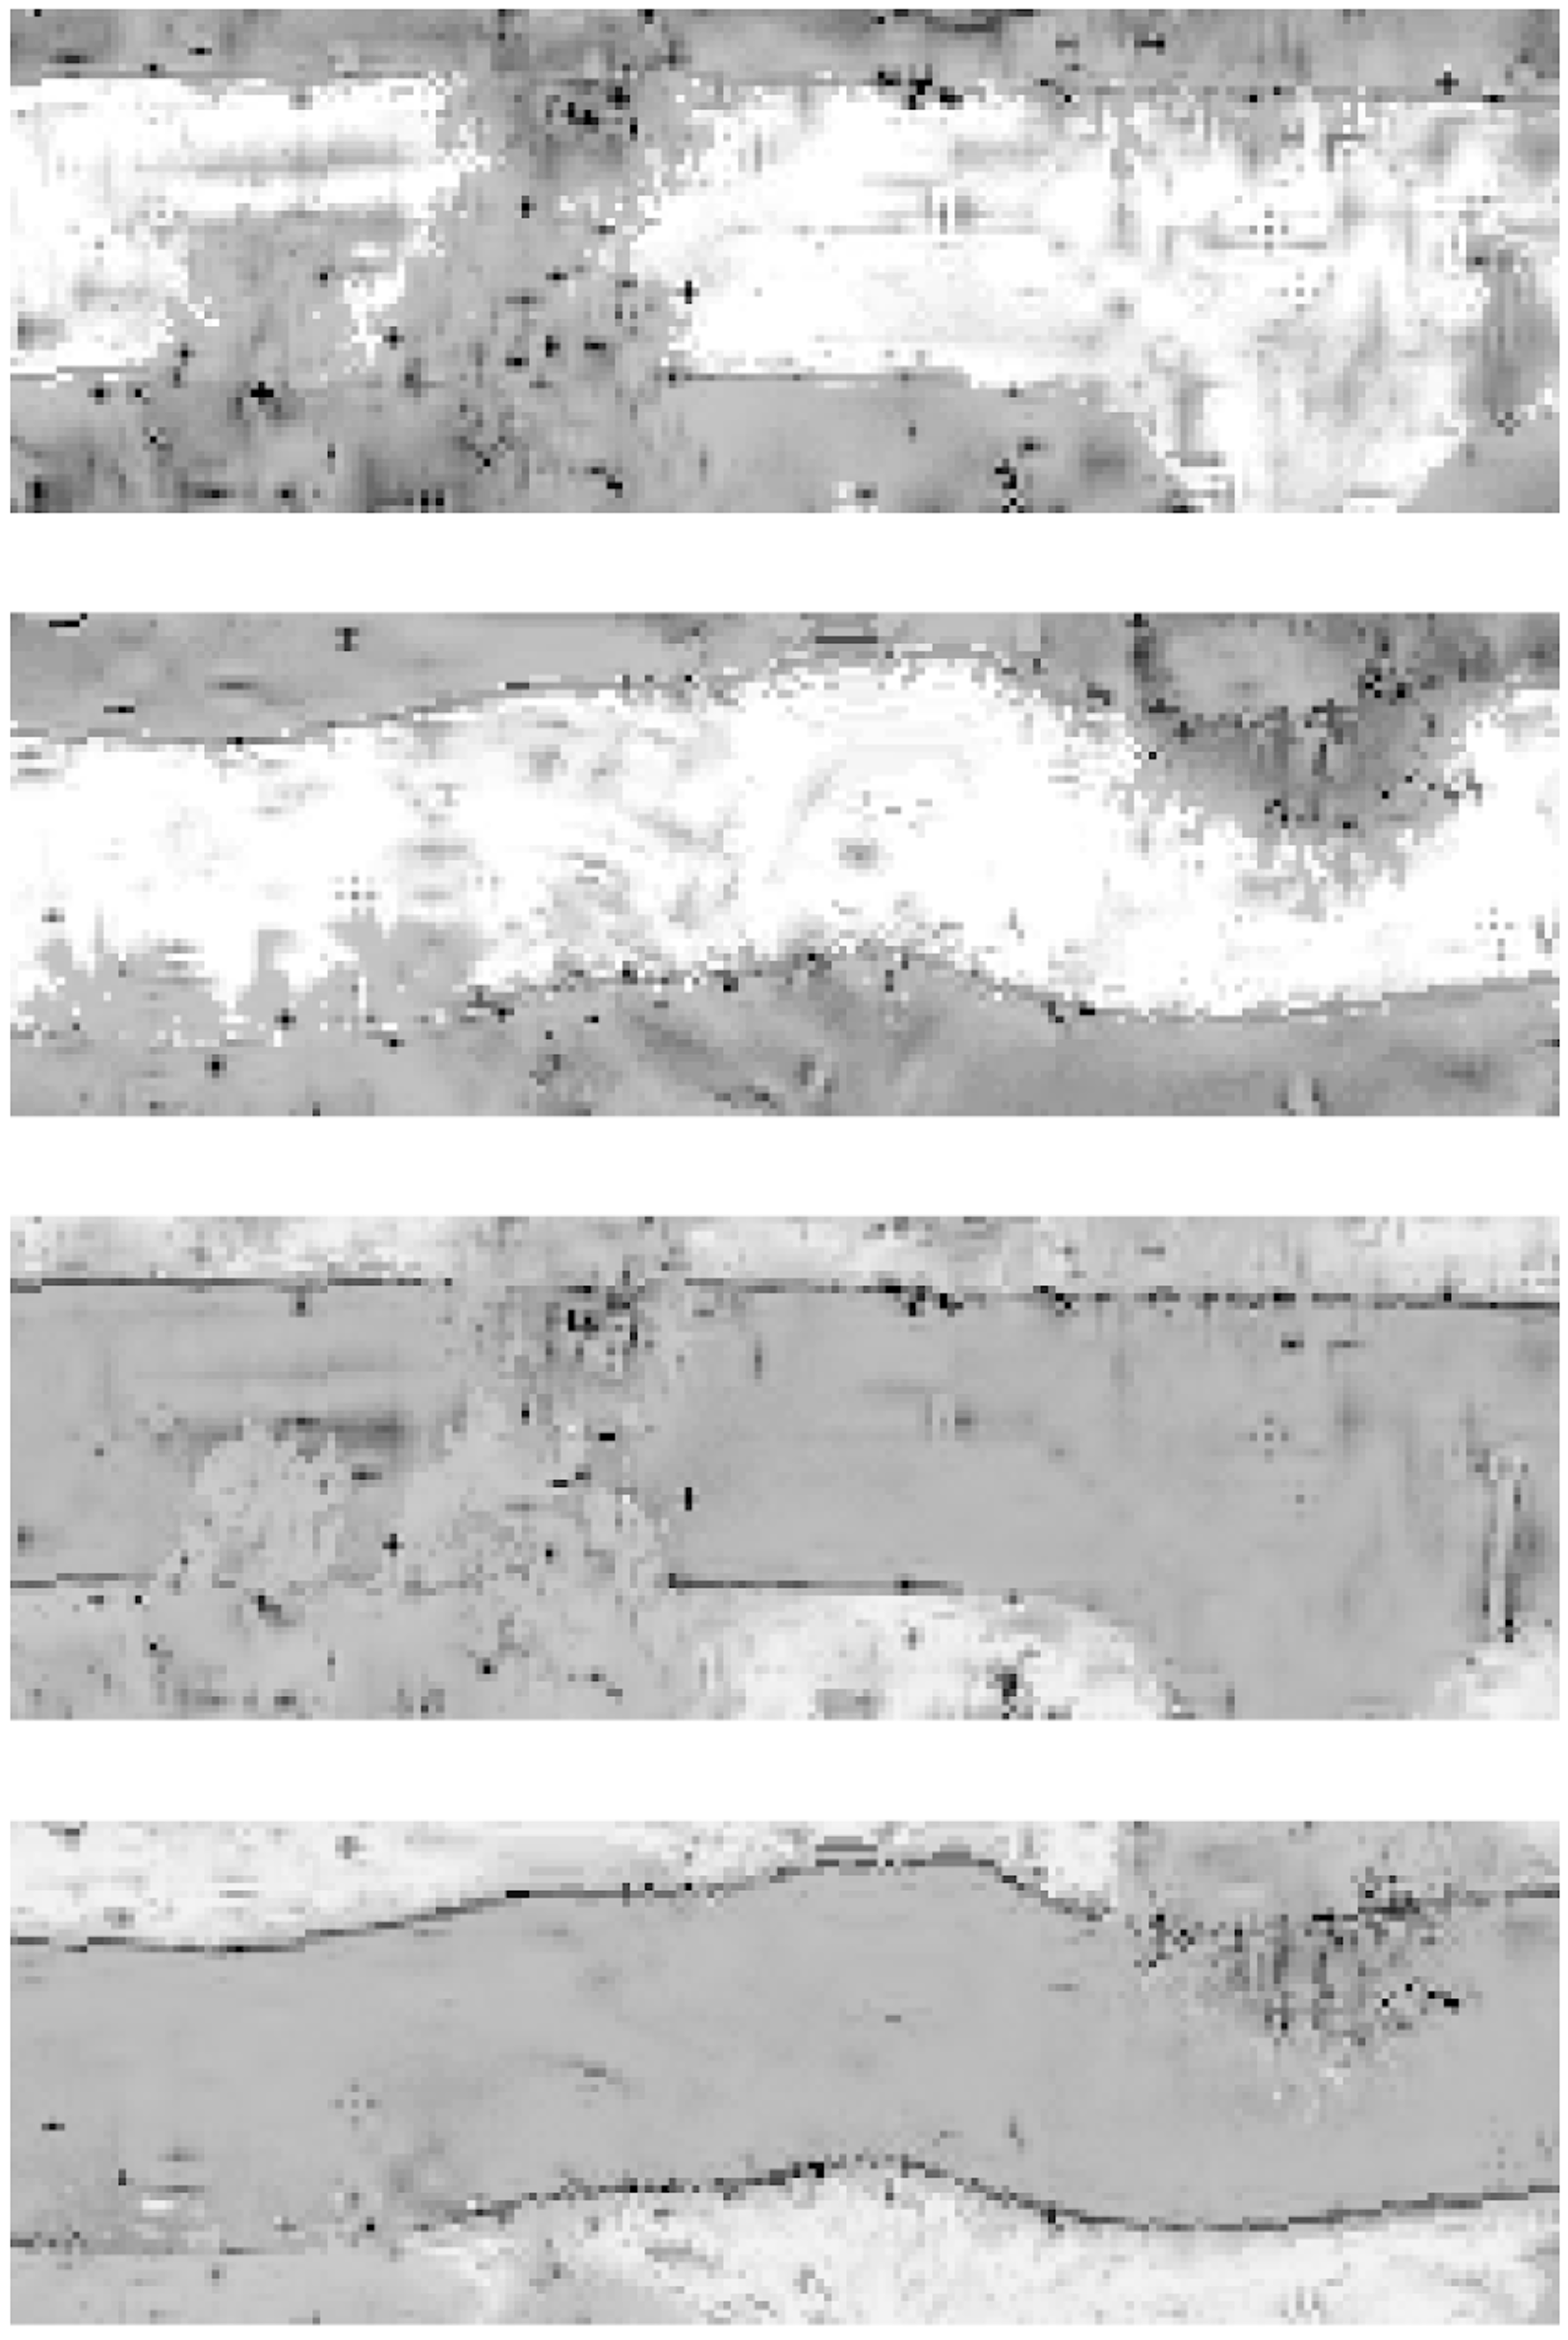
\includegraphics[width=0.6\columnwidth]{Figures/GMM_sample6.png}
    \caption[\ac{GMM} Result 2]{Example of GMMs on sample sidewalk. Row 1 and 2 shows the foreground GMM for sample sidewalk, and row 3 and 4 shows the back-ground for simple sidewalk. We use grey-scale to show the changes of probabilities, where for foreground, white is more likely to be sidewalk, and black is not.}
    \label{fig:GMM_result_2}
\end{figure}

We do not in general have a reliable estimate for the initial radius of our ribbon, but we can construct a trimap (\figref{fig:ribbon_3d}, bottom), as is done by \GrabCut{}, in order to estimate $\theta$. 
We choose a distance $\MaxDistance$ and numbers $\MinRadius < \MaxRadius$ so that all pixels with a distance of $[0, \MinRadius)$ are likely part of the ribbon (positive), all pixels within a distance of $[\MinRadius, \MaxRadius)$ are unknown, and others are are assumed not to be part of the ribbon (negative);
In our experiments we chose  $\MaxRadius$ as twice the expected mean width of ribbons (e.g. 2 meters), $\MinRadius = \MaxRadius/2$, and $\MaxDistance=\MaxRadius+\MinRadius$.  
In figure \ref{fig:ribbon_3d} these regions correspond to strips of pixels in $\RibbonImage{}$ along the edges and center of the image.

% \begin{figure}[h!]
%     \centering
%     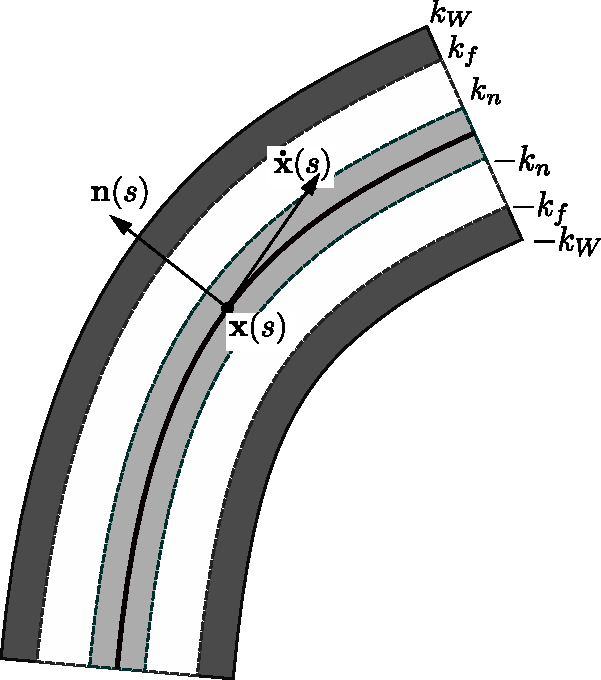
\includegraphics[width=0.3\textwidth]{Figures/sw-figure.pdf}
%     \caption[2D Ribbon Image]{A demonstration of the parameters for a ribbon in 2D, where $k_n$ indicates a lower-estimate for the radius of the ribbon, $k_f$ is an upper estimate, and $k_W$ is the maximum width of the ribbon image.}
%     \label{fig:2d_ribbon}
% \end{figure}

We use the EM-GMM algorithm to find a max-likelihood estimate of $\theta$ as a pair of Gaussian mixtures so that $\Pr(\Color{}|R, \theta)$ is a mixture of four multivariate Gaussian functions and $\Pr(\Color{}|\neg R, \theta)$ is a mixture of eight; then $\Pr(R|\Color{}, \theta)$ can easily be found using Bayes theorem as 
$$\Pr(R|\Color{}, \theta)= \frac{\Pr(\Color{}|R, \theta)}{\Pr(\Color{}|R, \theta)+\Pr(\Color{}|\neg R, \theta)}.$$



%\FloatBarrier

The resulting probabilities are illustrated in \figref{fig:GMM_result_2}; we observe that even a
coarse initial trajectory is usually enough to learn a more detailed, but noisy, estimate for the
foreground object shape. However colors alone are not able to discriminate between occlusion and
camouflage regions (such as the driveway in \figref{fig:GMM_result}).
Then the \ac{NLL} of a ribbon is proportional to a sum of $-\ln \Pr(R|\RibbonImage{}[i,j])$
for all $i,j$ within the ribbon and $-\ln \Pr(\neg R| \RibbonImage{}[i,j])$ for all $i,j$ outside the ribbon.
 The aim of our
\ac{DP} solution is to simultaneously optimize the probability based on color and shape of a
ribbon-like feature.

As shown in figure \ref{fig:GMM_Sample_2}, we applied a density estimation function to find the probability 
$\Pr(R|\RibbonImage[i,j])$ for each pixel in the ribbon image. 
For foreground density, we show the the probability likely-hood for 
the sidewalk-feature as gray-scale values, where white is more likely to be sidewalk and black is less likely. 
%We use the log likelihood function to calculate the foreground and background density and estimate density on pixels.

\begin{figure}[H]
    \centering
    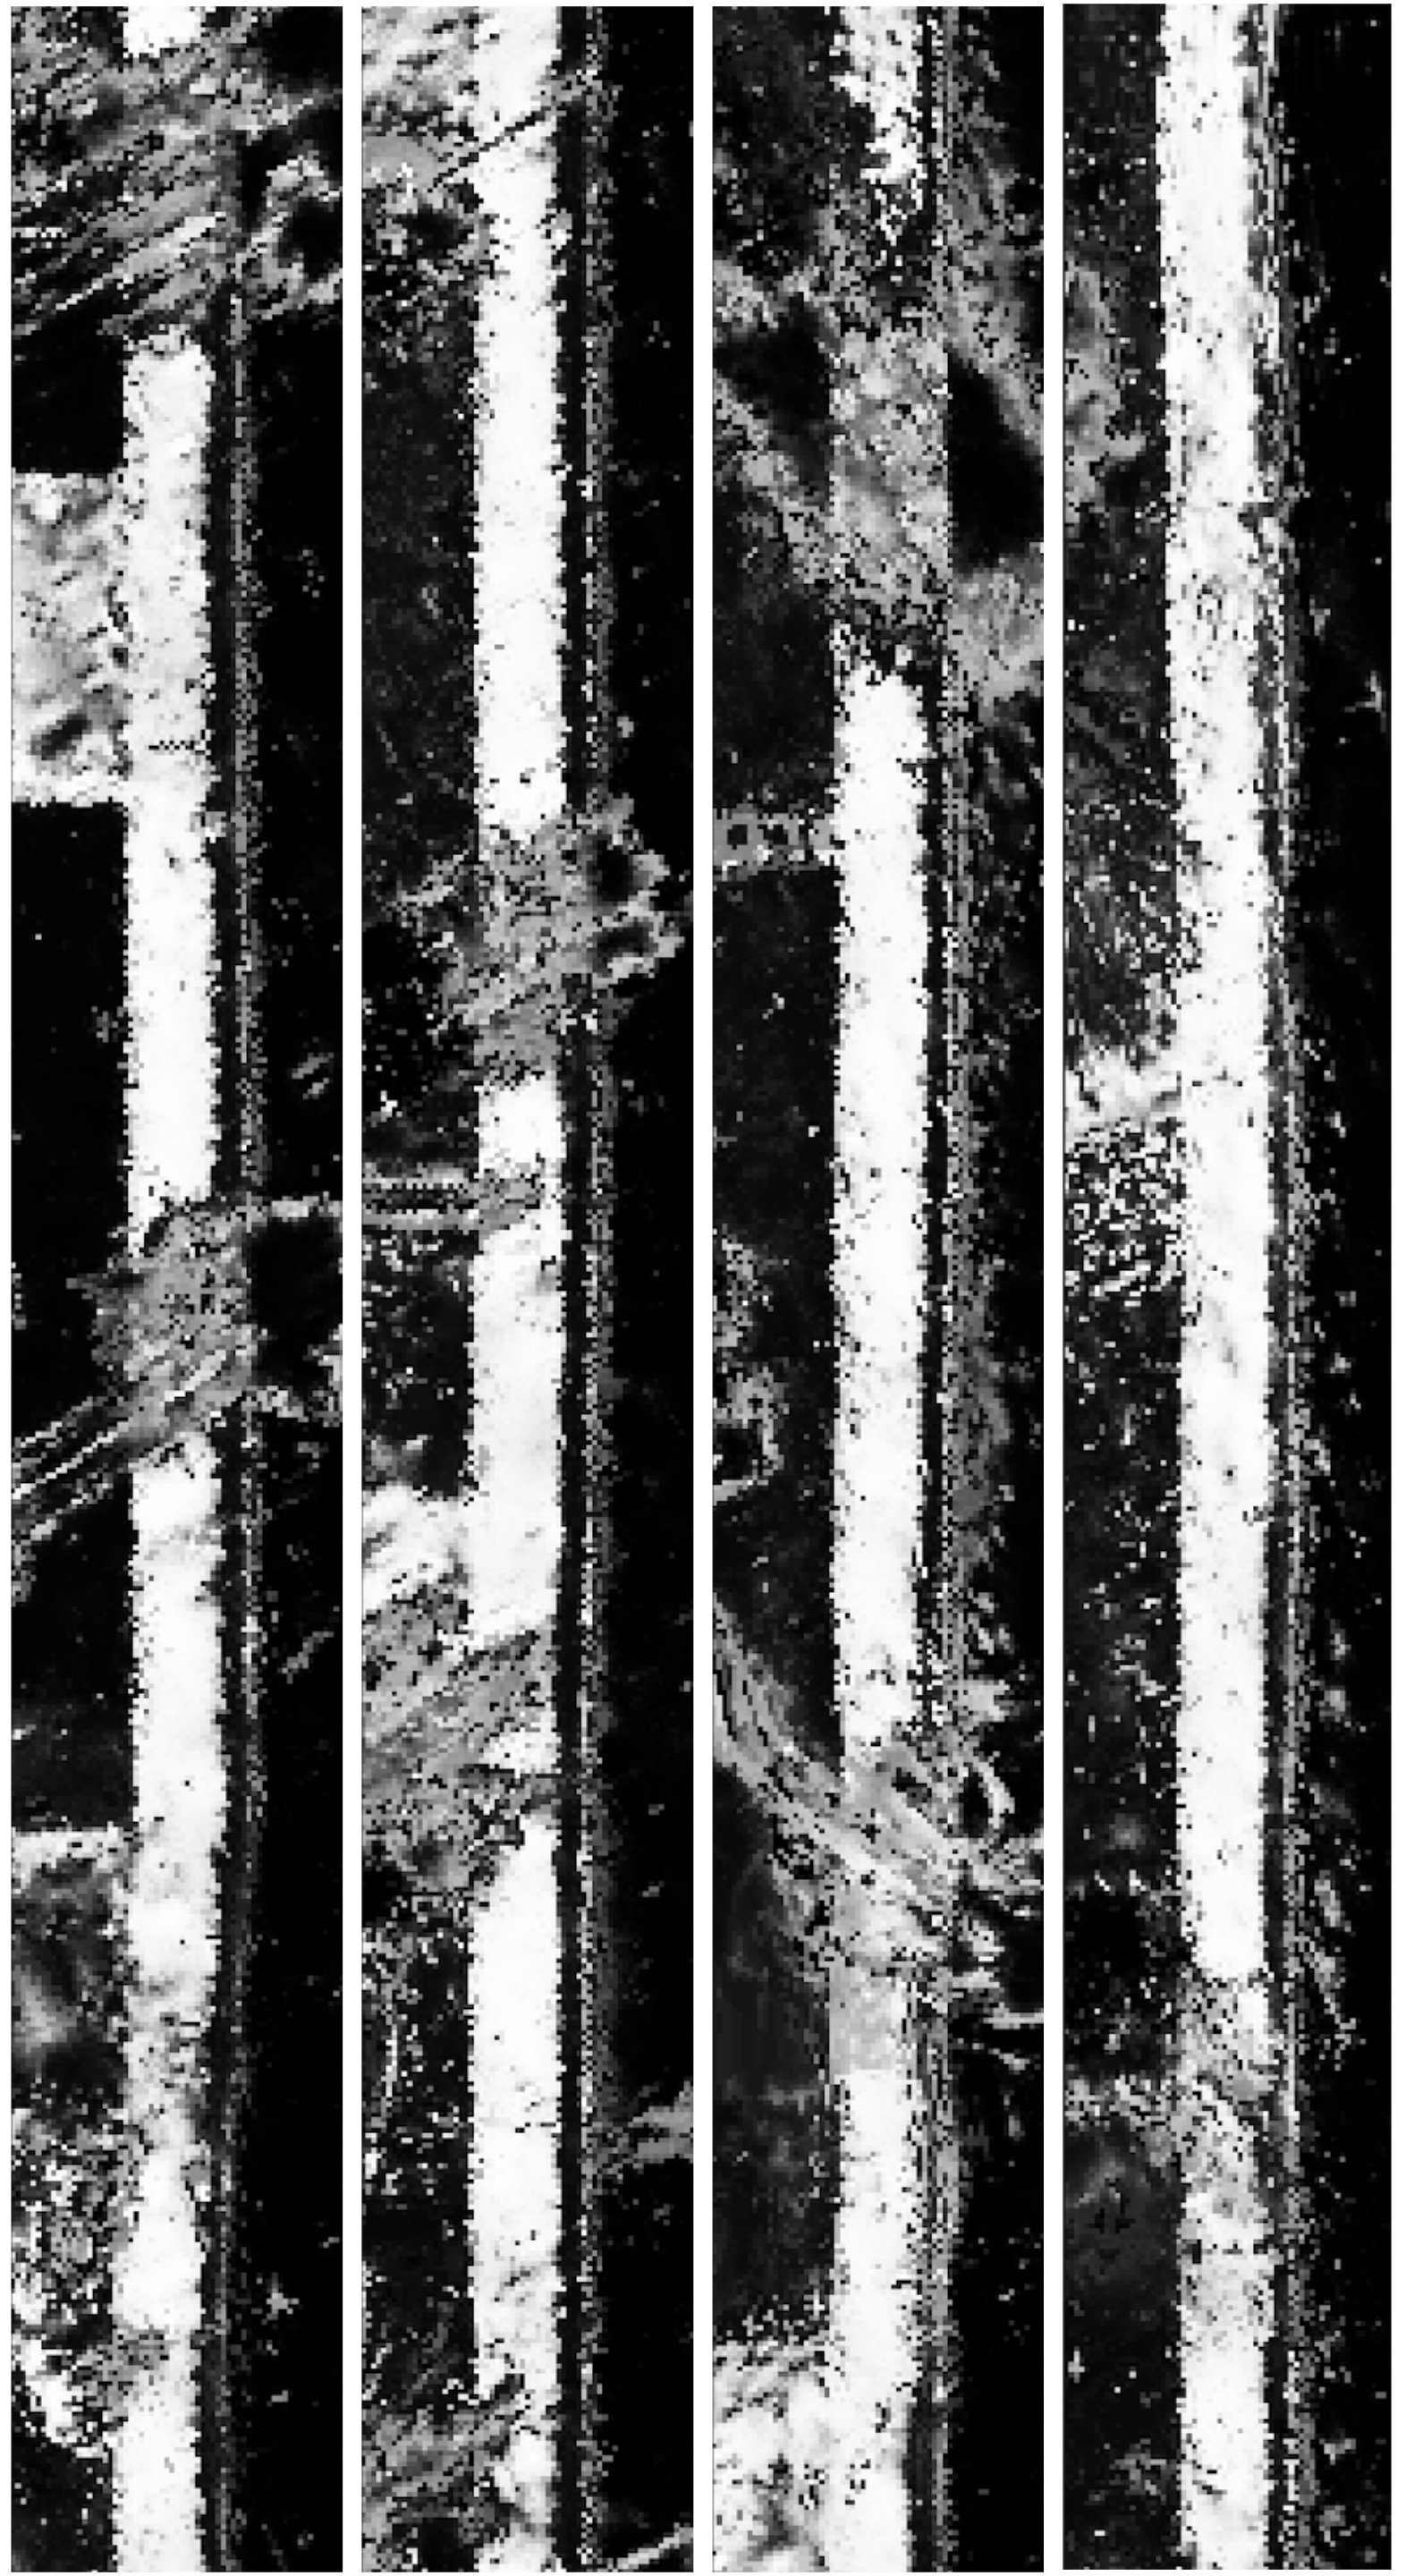
\includegraphics[width=\textwidth]{Figures/GMM_SAMPLE2.png}
    \caption[Density Estimation on Sample Sidewalk]{
    A sample figure with density estimation applied on figure \ref{fig:Sample_Sidewalk_2}. Where
    white indicates pixels are more likely to be a sidewalk feature and black indicates pixels are
    more likely to be a non-sidewalk feature. We separate it into 4 parts from column 1 to 4.}
    \label{fig:GMM_Sample_2}
\end{figure}


\section{A Dynamic Programming Algorithm}

We take $\RibbonImage{}$ as an input ribbon image with $m$ rows and $n=2\MaxDistance+1$ columns; $\RibbonImage{}{[i,j]}$ is a pixel in the image. 
We have an estimate $\Pr(R|\RibbonImage{}_{[i,j]}, \theta)$ which we abbreviate as $p_{[i,j]}$. 
In addition there is some small set of allowed perturbations $\delta=\{(\delta_j, \delta_k)\}$ where $\delta_j$ is a change in direction and $\delta_k$ is a change in the radius of the ribbon. 
Each perturbation has a probability $\Pr(\delta_j, \delta_k)$ that controls the shape of the curve; in our experiments we use $\delta_j\in\{-1,0,1\}, \delta_k\in\{-1, 0,1\}$ in order to ensure that results are connected, and  $\Pr(\delta_j, \delta_k)=\Pr(|\delta_j|)\Pr(\delta_k)$ is two independent multinomial distributions which require only three parameters due to symmetry and because probabilities sum to unity. 
We can interpret $c_\mathit{bend}=-\lg \Pr(\delta_j=\pm1)$ as a penalty for bending the curve, and $c_\mathit{shrink}=-\lg \Pr(\delta_k=-1)$ as a penalty for shrinking the radius, or $c_\mathit{expand} = -\lg \Pr(\delta_k=1)$ as a penalty for expanding the radius of the curve. 

% \begin{figure}[H]
%     \centering
%     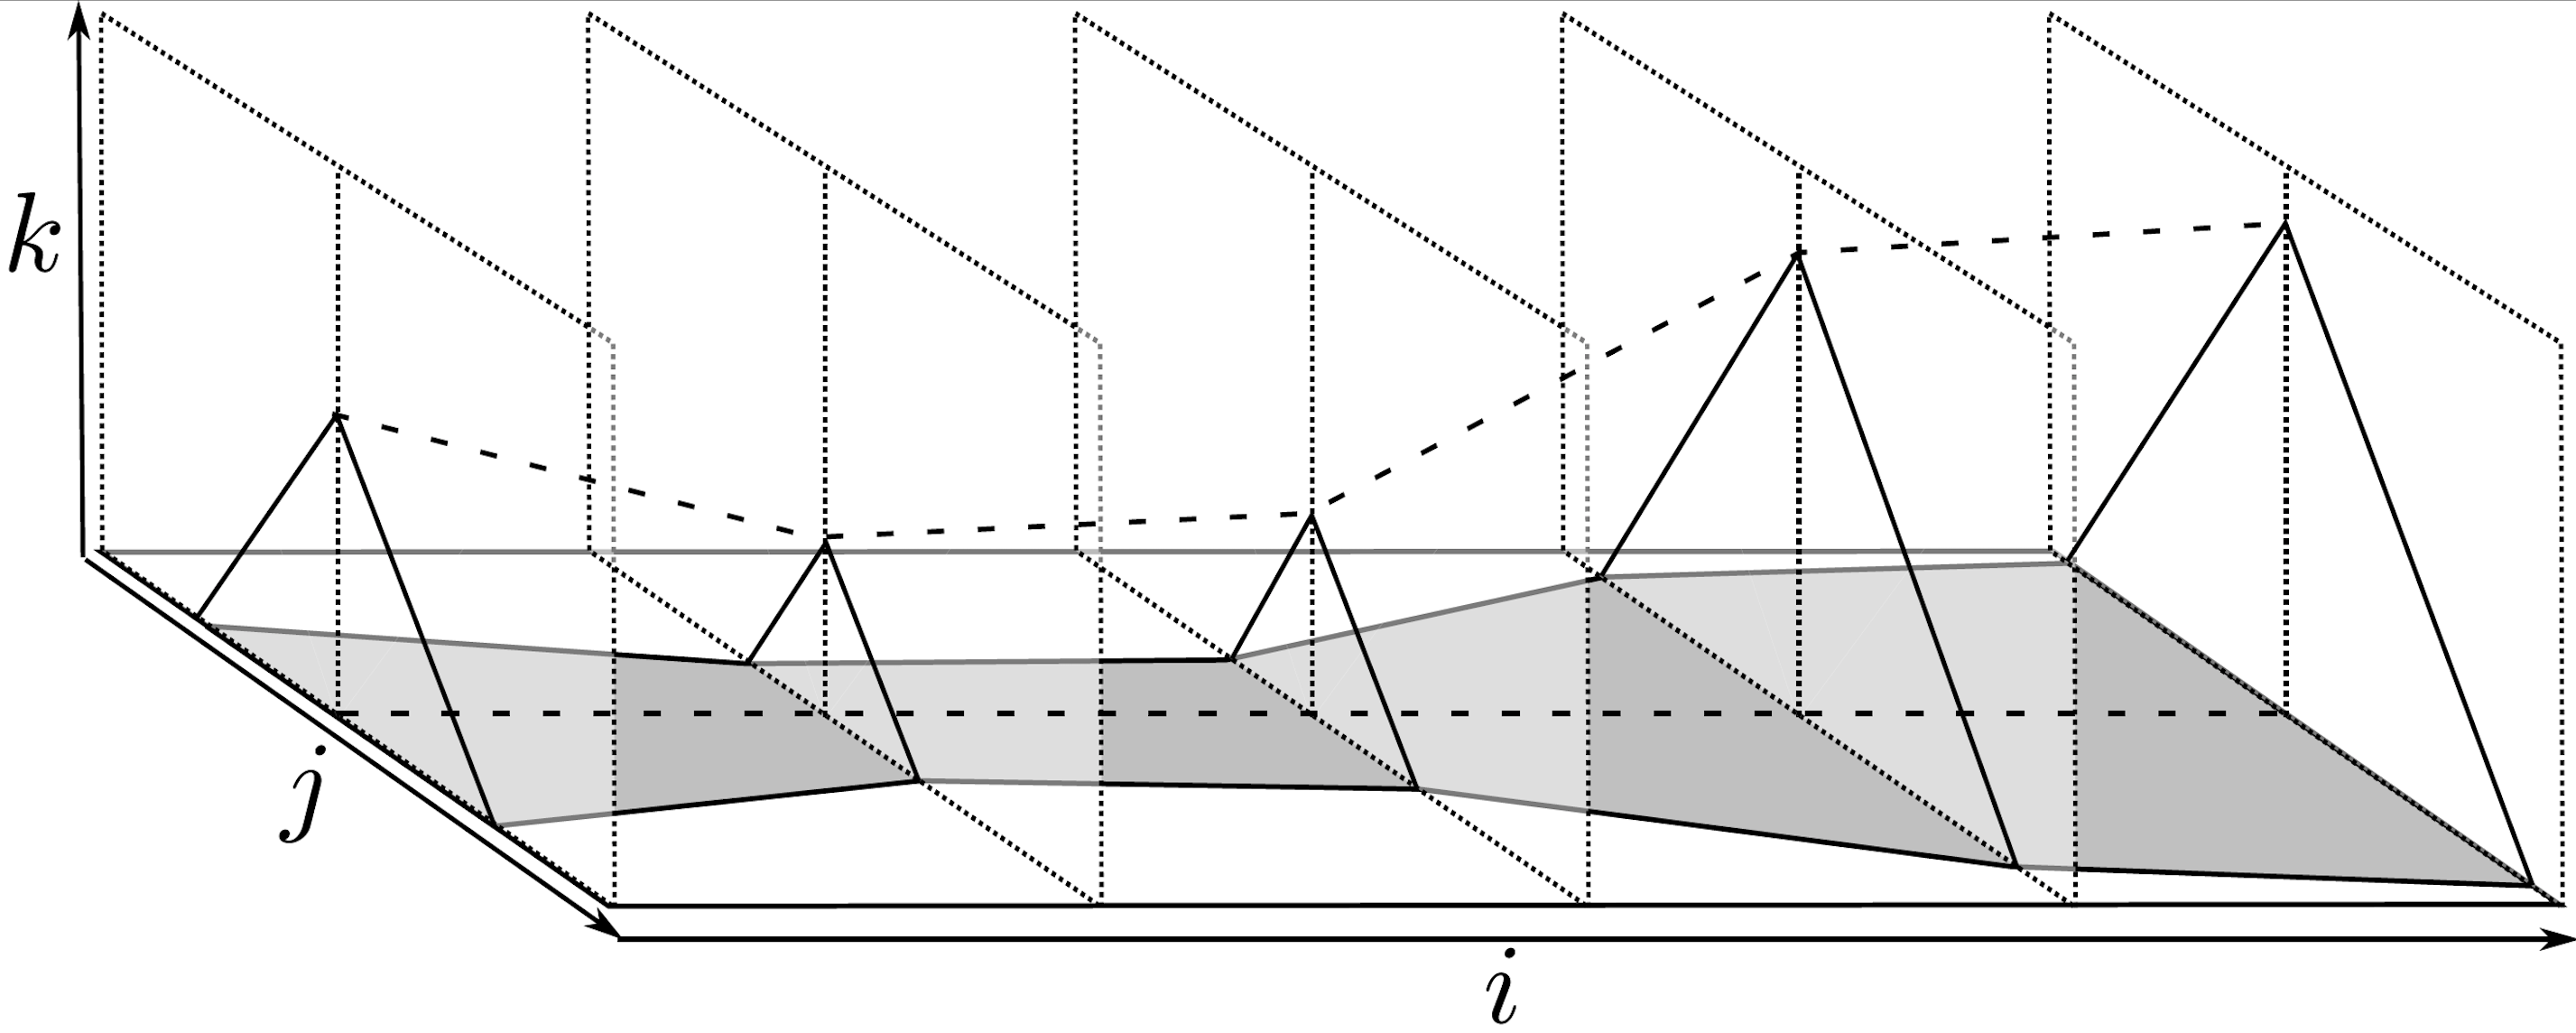
\includegraphics[width=\textwidth]{Figures/3dcombine_top.png}
%     \caption[3D Ribbon Image]{An illustration of the parameters for a ribbon: the $k$ axis captures the thickness of the ribbon and the $i$ axis captures the distance along the initial ribbon, the $j$ axis records horizontal displacements from the initial ribbon's medial curve.}
%     \label{fig:3d_ribbon_top}
% \end{figure}

We visualize the problem of finding a ribbon as one of choosing a three-dimensional path through a scale-space where the first two dimensions represent locations of the ribbon's center, and the third dimension represent the thickness of the ribbon as illustrated in \figref{fig:ribbon_3d}. Every ribbon must start at one end of the image and follow a three-dimensional path through scale-space to reach the other end one slice at a time. Each slice corresponds to a row of the ribbon image and a point at location $(j, k)$ in the slice partitions the row into negative regions $(0\twodots{}j-k-1)$ and $(j+k+1\twodots{}n)$ with a positive region at $(j-k \twodots{} j+k)$ with thickness $2k+1$. The likelihood of any location $(j, k)$ is the product of the probabilities that each pixel on the same row belongs to the corresponding positive or negative regions.  In fact the probability is exponentially related to the size of each pixel; if one were to increase the resolution by a factor of $r$ then the contribution of each pixel would be raised to the power of $\frac{1}{r}$ so that the product would stay constant. In order to make our parameters invariant to scale, we divide the \ac{NLL} by $\MaxDistance{}$ when estimating the likelihood of a given $(j,k)$. 

We model the probability of a ribbon as the product of the probability of each location $(i, j, k)$ along the path times the probability of each edge from slice $i$ to slice $i+1$. We use dynamic programming to search to a path that minimizes the \ac{NLL} (the cost) of a path in procedure \proc{Segment-Ribbon}.

The pseudocode can be interpreted as follows: Line \ref{li:loop-slices} iterates through each slice of the ribbon image. Line \ref{li:loop-radius} iterates through all possible radii and line \ref{li:loop-center} explores all possible ribbon-centers from left to right. We use a variable $s$ to calculate \ac{NLL} of a set of regions as the ribbon shifts from left to right. If this is not the first slice, then line \ref{li:min-from-pred} selects the least-expensive (most probable) path that leads to location $(i, j, k)$ in the scale space.  At each step on pixel toggles from negative to positive, and one toggles from positive to negative as $s$ is updated in line \ref{li:update-s}.  We return the costs as well as the final offset and scale $(j^*, k^*)$ of the best path. 


\begin{codebox}
\Procname{$\proc{Segment-Ribbon}(\RibbonImage{})$} \label{alg:segmet-ribbin}
\li $p[i,j]\gets -\lg \Pr(\RibbonImage{}[i,j])/\MaxDistance{}$, 
          \hspace{2ex} $q[i,j] \gets -\lg \Pr(1-\RibbonImage{}[i,j])/\MaxDistance{}$
\li $C{[0\twodots{}m, 0\twodots{}n, 0\twodots{}n]} \gets \infty$
\li \For{$i \gets 0 \To m$} \Do                                                \label{li:loop-slices}
\li     \For $k \gets 0 \To \lfloor n/2 \rfloor $ \Do                          \label{li:loop-radius}
\li         $s = \displaystyle{\sum_{j=0}^{2k} p[i,j] +\sum_{j=2k+1}^n  q[i, j] }$
\li         \For $j \gets k \To n-k$ \Do  \label{li:loop-center}
\li              \If $i > 0$  \Do                                              \label{li:if-has-pred}
\li              $v \gets s {+}\displaystyle{\min_{\delta_j, \delta_k}\left(  
                              C[i{-}1,j{+}\delta_j,k{+}\delta_k] -\lg \Pr(\delta_j, \delta_k)
                            \right)}$  
                               \label{li:min-from-pred}
\li              \Else $v\gets s$
                 \End
\li              $C{[i, j, k]} \gets v$                                       \label{li:dp-store}
\li              $s \gets s{+}q[i,j{-}k]{-}p[i, j{-}k]{+}p[i, j{+}k]{-}q[i,j{+}k]$ \label{li:update-s}
           \End
       \End
    \End
\li $j^*, k^* \gets \displaystyle{\arg\min_{j,k} C{[m, j, k]}}$
\li \Return $C, j^*, k^*$
\end{codebox}

The \proc{Backtrack-Ribbon} algorithm selects the least-costly (most probable) ribbon and it is
copied into to \OutputTrajectory{} and \OutputRadius{};
so that the most likely path has scale-space coordinates $(i, \OutputTrajectory{}[i],
\OutputRadius{}[i])$ for $i=0\twodots{}m$.



\begin{codebox}
\Procname{$\proc{Backtrack-Ribbon}(C, j^*, k^*)$} \label{alg:backtrack-ribbon}
\li $\OutputTrajectory{}{[0{\twodots}m]} \gets 0$, \quad $\OutputRadius{}[0{\twodots}m] \gets 0$             
\li $\OutputTrajectory{}{[m]}, \OutputRadius{}{[m]} \gets j^*, k^*$ \label{li:backtrack-best-last}
\li \For $i \gets m-1 \Downto 0$ \Do
\li      $\delta_j, \delta_k = \displaystyle{\arg\min_{\delta_j,\delta_k}C{[i,j{-}\delta_j,k{-}\delta_l]}{-}\lg \Pr(\delta_j,\delta_k)}$
\li      $\OutputTrajectory{}{[i]}, \OutputRadius{}[i] \gets \OutputTrajectory{}{[i+1]}-\delta_j, R{[i+1]}-\delta_k$                                                 \label{li:backtack-choose-pred}
    \End
\li \Return $\OutputTrajectory{}, \OutputRadius{}, C_{[m, j^*, k^*]}$
\end{codebox}


If one wishes the path to be connected in scale-space, then there are only $3\times3$ possible values for $\delta_j, \delta_k$ in line \ref{li:min-from-pred}; so the algorithm is $\Theta(m n^2)$ and used $O(m n^2)$ space, where $m$ is the length of a ribbon and $n=2\MaxDistance+1$ is the maximum thickness of a ribbon. Since $\MaxDistance$ is typically a constant, this algorithm is effectively linear on the length of a ribbon.

%We use our dynamic programming algorithm on the ribbon image to find the max score for each pixel that had better probability to be sidewalk feature that we mentioned in Chapter 4. 
%More importantly, we introduce a penalty control function that makes each horizontal movement in the edges or center cost more than vertical movement. Basically, for each line of pixels, if they think the edges or center should shift more horizontally than one pixel compares to the last line, we score them with more penalty. 

Figure \ref{fig:penalty} shows our algorithm managed to separate the driveway and sidewalk under the same feature as penalty increase. So we could apply the dynamic programming solution to locate the precise boundaries of given ribbon image. The penalty control improved our performance significantly. Because of this, our approach could predict the sidewalk under the tree shadow and other shadows or obstacles, which bring us more accurate result compare to other methods.
\begin{figure}[H]
    \centering
    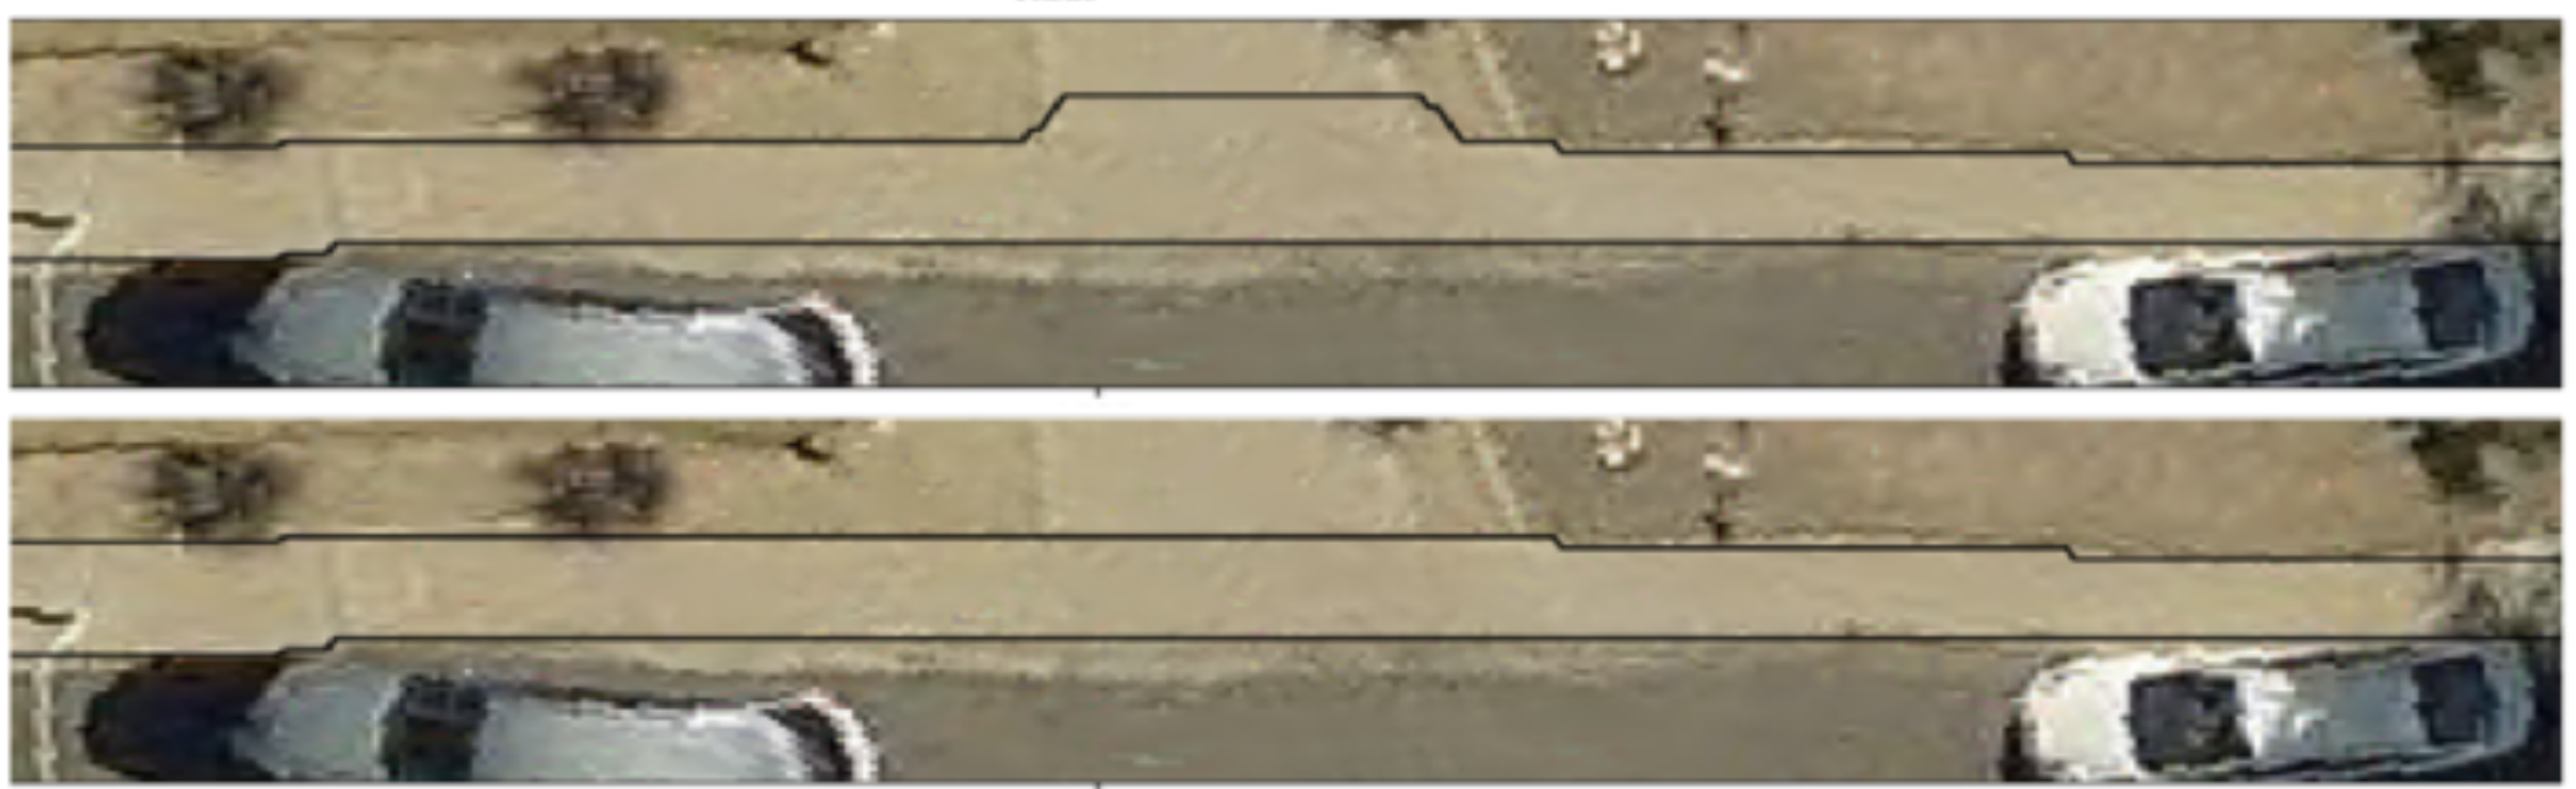
\includegraphics[width=\textwidth]{Figures/penalty.png}
    \caption[Penalty Process]{Comparison with penalty change, we tested a variety of variables to decide which variable had best performance for width control. With the penalty increased at a reasonable amount, our algorithm decided not to recognize a driveway as sidewalk walk, in order to keep the sidewalk width consistent, even though they are the same texture.}
    \label{fig:penalty}
\end{figure}

As shown in figure \ref{fig:sample_result2}, after we generate the result on ribbon image, just need to simply covert the ribbon image back to its original shape by reverse the method that generates the ribbon image. 

\begin{figure}[H]
    \centering
    \includegraphics[width=0.95\textwidth]{Figures/sample2_result.png}
    \caption[Desire Output on Sample Sidewalk]{Detail demonstration on desire result after applying our dynamic programming approach. Where row 1 shows the result after reshape, row 2 to 5 shows the boundaries we calculated on ribbon image from \ref{fig:Sample_Sidewalk_2}.}
    \label{fig:sample_result2}
\end{figure}